% !Mode:: "TeX:UTF-8"

\chapter{基于深度学习的辐射源识别}
\label{sec:sei}
% TODO:增加内容与仿真!!!
% 对比利用不同的,添加具体参数的设置。


% 可以考虑进行未经过模糊函数处理和处理之后的对比

% 不同卷积核  学习率  不同卷积核个数
% 层数 节点数等
% 不同训练方法
% 多类别的分类结果图可以参考
% 不同数据的各自的图

\section{引言}
辐射源识别算法需要在无法收集大量数据的前提下正确的对目标进行分类并准确区分出已知目标和未知目标。
与传统利用已知类别的样本进行训练测试的机器学习算法不同,本站的问题是在Open Set的背景下,需要考虑输入未知分类样本的情况。
由于在复杂电磁环境下传统的辐射源个体识别面临识别能力差和无法识别未知目标等问题与挑战,因此需要寻找一种新的方法解决该问题。

本章综合雷达信号处理、深度学习等多学科理论,通过对实际数据的分析,结合深度卷积神经网络与支持向量机方法,以雷达信号的模糊函数切片作为训练样本的特征向量,构建了一个可以对未知分类进行辨识的分类器。最后,利用数据进行验证,证明本章提出的分类器具有很高的准确性。

本章安排如下: \ref{sec:sei_data}节对辐射源信号进行了分析,并对其进行预处理,求取其模糊函数切片,\ref{sec:sei_method}节构建了本章的Open Set 分类器,详细地阐述了深度卷积神经网络主分类器与支持向量机Meta-Recognition的设计过程,\ref{sec:sei_experiment}节利用数据对分类器已知分类识别和未知分类辨别的性能进行了验证,\ref{sec:sei_summary}节进行本章总结。

\section{辐射源信号分析}
\label{sec:sei_data}
对辐射源信号的分析处理,本章主要考虑两方面:信号预处理、特征提取优化。
本章所获得的信号为雷达辐射源的I/Q两路数据,这是一种在雷达信号处理领域常见的用来描述信号的方法。其中I表示In-Phase,即同相;Q表示Quadrature,即正交,与I相位之差为90度。
设需要表示的信号的峰值幅度为$A$、相位角为$\phi$,则有:
\begin{equation}
	I = A\cos{\phi},
	\label{equ:i}
\end{equation}
\begin{equation}
	Q = A\sin{\phi}.
	\label{equ:q}
\end{equation}
也即可以利用\equref{equ:signal}表示信号:
\begin{equation}
	Ae^{i\phi}=A(\cos(\phi) + i\sin(\phi))=I+Qi.
	\label{equ:signal}
\end{equation}
从而可以根据\equref{equ:i}和\equref{equ:q}利用I/Q数据求取信号的峰值幅度和相位角:
\begin{equation}
	A=\sqrt{I^2+Q^2},
\end{equation}
\begin{equation}
	\phi=tan^{-1}(Q/I).
\end{equation}
在完成信号形式的转换后,首先需要对信号进行初步的预处理,剔除无用和错误的数据。
在特征提取优化方面,合理的特征是分类识别的基础。由于存在相同型号的辐射源,利用简单的参数特征无法很好的完成辐射源的个体识别,但是在实际中辐射源自身存在相位噪声以及各类杂散输出,此部分特征可以用来区分出型号、参数均相同的辐射源,因此需要选取一种可以提取雷达辐射源这种无意调制产生的信号脉内细微特征的方法。
模糊函数不仅能描述辐射源信号的分辨特性与模糊度,还能描述由雷达辐射源信号所决定的测量精度、杂波抑制特性等,通过模糊函数在时延和频偏这两个维度上的变换,可以多角度的刻画出无意调制对发射信号的影响,最终选取了利用雷达模糊函数挖掘辐射源的特征。
\subsection{模糊函数}
信号$x(t)$的瞬时自相关函数为$R_x(t,\tau)=x(t+\tau/2)x^{*}(t-\tau/2)$,其中$\tau$为时延,模糊函数的定义为,
\begin{equation}
A(\tau,\nu) = \int_{-\infty}^{+\infty}R_x(t,\tau)e^{j2\pi\nu t}dt,
\label{equ:defineaf}
\end{equation}
即$R_x(t,\tau)$关于时间$t$的傅里叶反变换。

为了方便在数字信号中使用,\equref{equ:defineaf}可以经过变换等价于\equref{equ:afcon}的形式:
\begin{equation}
A(\tau,\nu) = \int_{0}^{\tau}x(t)x^{*}(t+\tau)e^{j2\pi\nu t}dt.
\label{equ:afcon}
\end{equation}
对信号均匀采样,即对接收信号和参考信号离散化后,\equref{equ:afcon}可以表示为:
\begin{equation}
A(\tau_l,\nu_m) = A(l, m) = \sum_{n = 0}^{N-1}x(n)x^{*}(n+l)e^{\frac{j2\pi m n}{N}},
\end{equation}
其中,$\tau_l=l/f_s$、$\nu_m=mf_s/N$。

此处以一个简单的单载频矩形脉冲信号来展示模糊函数特征提取的作用,图\ref{fig:danpinmaichong}为模糊函数图,可以发现模糊函数存在一定的冗余,其主要变化均处于0时偏和0频偏附近。
为了减小计算量,本章在频偏为0附近取不同时间延迟的切片作为信号特征,可以有效地提取信号的相位噪声和杂散输出等个体特征,并且此处受噪声的干扰较小,更加稳定。图 \ref{fig:qiepian}即为在频偏为0处的单载频矩形脉冲信号模糊函数切片。

\begin{figure}[hbt]
	\centering
	\begin{minipage}[b][][b]{7cm}
		\centering
		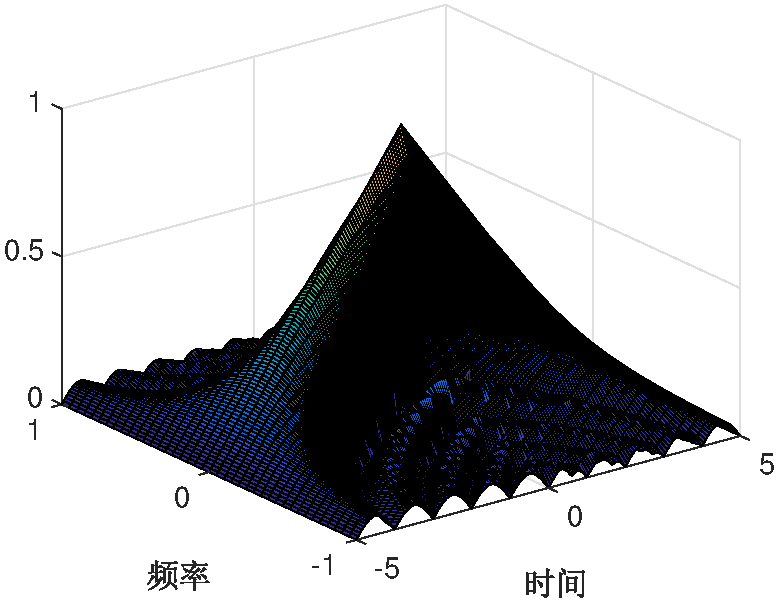
\includegraphics[width=6.67cm]{figures/emitter/danpinmaichong}
		\caption{单载频矩形脉冲信号模糊函数图}
		\label{fig:danpinmaichong}
	\end{minipage}
	\hspace{10pt}
	\begin{minipage}[b][][b]{7cm}
		\centering
		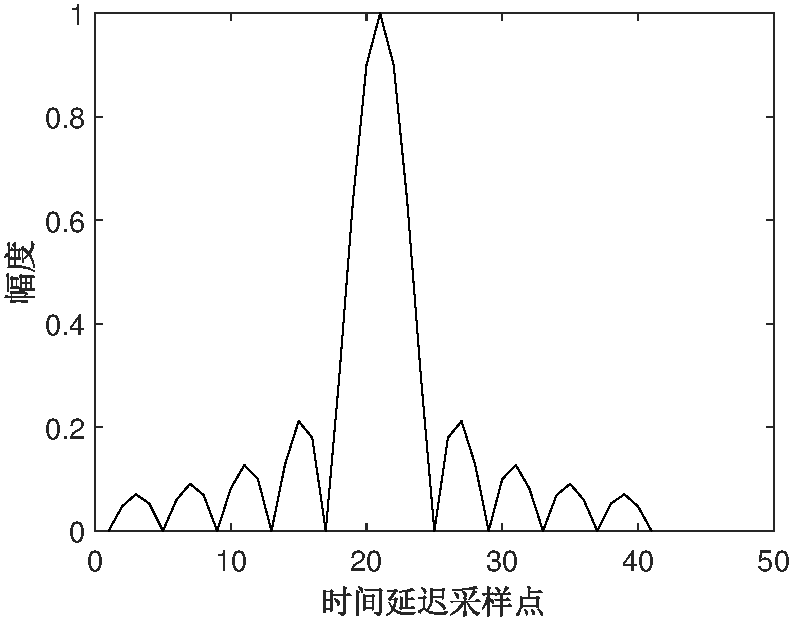
\includegraphics[width=6.67cm]{figures/emitter/qiepian}
		\caption{单载频矩形脉冲信号模糊函数切片}
		\label{fig:qiepian}
	\end{minipage}

\end{figure}

\section{Open Set 分类器设计}
\label{sec:sei_method}
通常的识别或者分类系统仅考虑的是一个闭集分类系统,然而在现实世界中,这种分类系统会遇到很大的问题。由于其最基本的假设是所有的类别均为先验已知,那么就会出现问题,例如在训练样本中不存在类别的样本就会被错误的分到某个类别中去。这种在训练过程提供不完整的信息,而在测试时添加未知分类的问题,称作Open Set识别\ucite{scheirer2013toward, jain2014multi}。该问题还可以描述为需要在测试过程中拒绝未知样本,Open Set目标识别系统必须可以准确的处理以下三种类型的数据类:
\begin{itemize}
	\item 已知的(目标)类,被标注为正训练样本的数据,
	\item 已知的未知(非目标)类,被标注为负训练样本的数据,
	\item 未知的未知(非目标)类,在训练样本中不存在的类别的数据。
\end{itemize}
传统的机器学习算法均是针对闭集数据设计的,随着识别算法应用场景的增多和对精度要求的提高,许多学者开始了对Open Set识别的研究。Simonson\ucite{simonson1998probabilistic}提出了一种称作概率融合(probabilistic fusion, PF)的利用统计的方法来进行Open Set识别,其主要通过合并来自不同数据源的证据得到一个统计测试模型,根据此模型的分布来对类别进行判断。Scheirer等人\ucite{scheirer2011meta}提出了一种通过分析后验数据得分来进行类型判断的方法。

此部分主要解决的问题是当得到一个新的测试样本,如果该样本不属于已经经过训练的分类,那么传统的神经网络模型会将该样本指派给与其最相似的一个类别,此种情况对一个Open Set识别系统,也即类似于辐射源识别系统这种具有较多尚未经过训练的样本的一个数据集,首先这会导致其识别率下降,另一方面是由于对未知辐射源无法很好的确定,无法很好的完成预警等任务。
目前,学者对该问题的研究主要有两个思路:
\begin{itemize}
	\item 在训练集中添加一个“未知”类别,利用不同的来自非已知类别的数据作为训练样本对该类别进行训练,然后对所有的输入数据进行类别的识别,将识别结果为该类别的数据作为未知分类数据。
	\item 针对多分类使用的softmax函数,可以设立阈值或者对该识别结果进行一个评价(例如与已知类别数据的一个“距离”),通过这种方式分辨出未知分类。
\end{itemize}
第一个思路最大的问题是实际工程中无法得到所有可能的未知类别的样本来进行训练,具有一定的局限性,不适用于本章这个具有大量来自未知分类数据的问题。针对该问题,本章基于后一个思路设计了一个基于Meta-Recognition的可以识别未知辐射源的深度神经网络。首先是创建一个深度卷积神经网络分类器,该分类器的输出为该训练样本属于各个类别的概率,然后将此类别作为一个输入,输入到一个支持向量机分类器Meta-Recognition中,然后利用该Meta-Recognition判断输入是否为未知分类。
\begin{figure}[hbt]
	\centering
	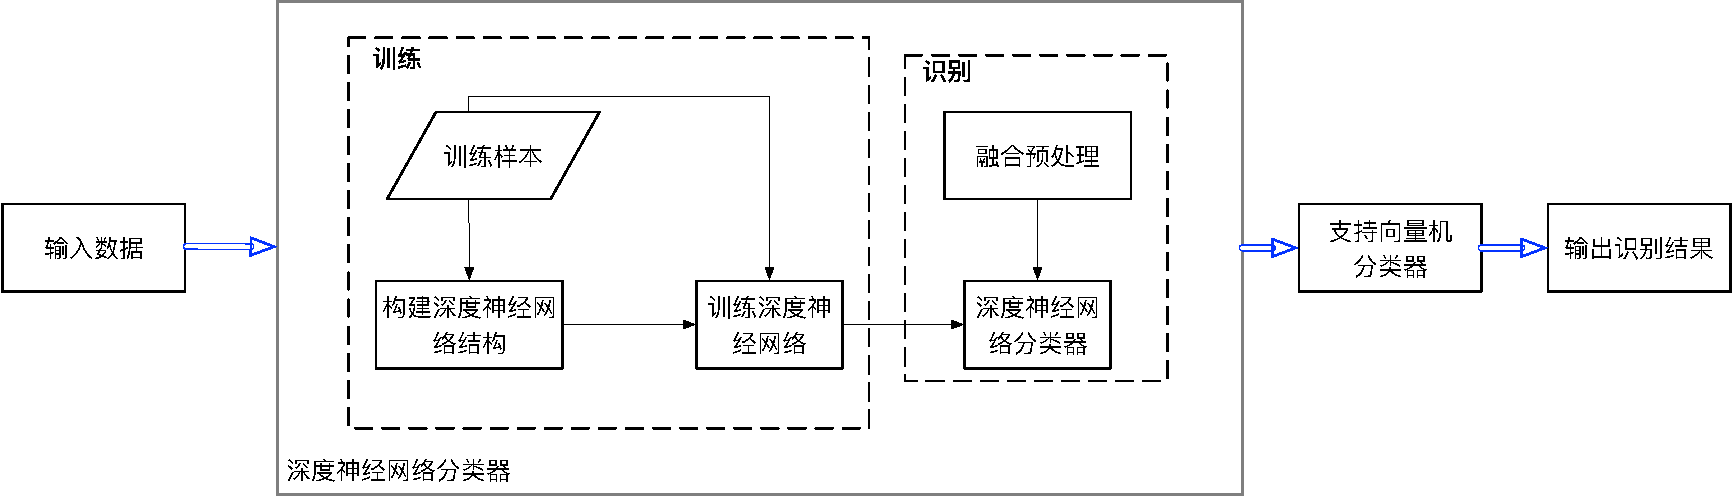
\includegraphics[width=13.5cm]{figures/emitter/frame_emitter}
	\caption{分类器设计结构图}
\end{figure}

\subsection{深度卷积神经网络分类器设计}
本章根据辐射源信号的实际数据以及其反映出来的特性,设计了一个如图\ref{fig:struct_emitter}所示具有10层的一维卷积神经网络。
该分类器作为主分类器,且Meta-Recognition是以该分类器的输出作为输入,所以该分类器性能的好坏会直接影响到对已知类别的分类和对未知类别的判断。

第一层是输入层,由于模糊函数切片为一个$1 \times 1000$的向量,因此输入层大小是$1 \times 1000$。

第二层是卷积层$C1$,$C1$对输入向量进行一维卷积运算提取特征,卷积运算可以最
大程度的提取原始信号的特征。此处利用了256个大小为$1\times 3$的卷积滤波器,其窗口移动步长为1。

第三层是一个池化层$S2$,$S2$层对上一层$C1$做池化处理,池化的目
的是在保留数据有用信息的同时,尽可能减少数据量。此处采用的是$1\times 2$的最大池化操作。

第四层是一个卷积层 $C3$,$C3$对$S2$的特征进行卷积操作,此处利用了128个大小为$1\times 3$的卷积滤波器。

第五层是一个卷积层 $C4$,其结构与$C3$相同,128个大小为$1\times 3$的卷积滤波器。

第六层是一个池化层 $S5$,其结构与$S2$相同,$1\times 2$的最大池化操作。

第七层是一个卷积层 $C6$,其结构与$C3$相同,128个大小为$1\times 3$的卷积滤波器。

第八层是一个卷积层 $C7$,其结构与$C3$相同,128个大小为$1\times 3$的卷积滤波器。

第九层是一个池化层 $S8$,其结构与$S2$相同,$1\times 2$的最大池化操作。

第十层是输出层,根据不同的类别个数选取相应的输出节点个数,首先将$S8$的特征拉成一个一维向量,然后通过全连接网络与输出层进行连接,通过Softmax激活函数输出最终的结果。

\begin{figure}[hbt]
	\centering
	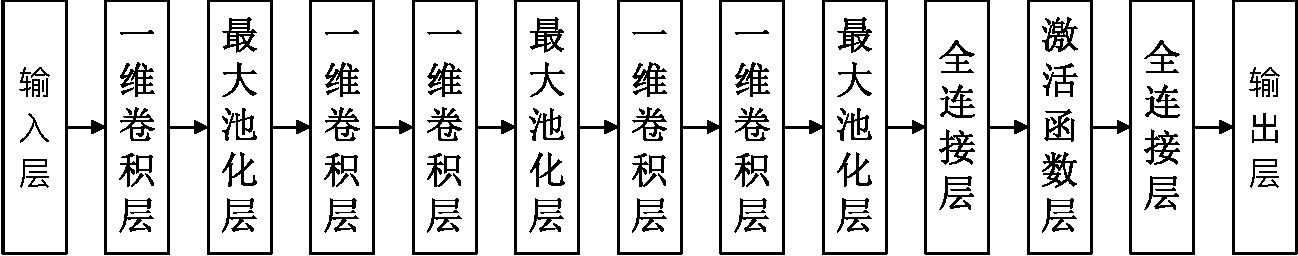
\includegraphics[width=13.5cm]{figures/emitter/struct_emitter}
	\caption{深度卷积神经网络框架图}
	\label{fig:struct_emitter}
\end{figure}

\subsection{支持向量机 Meta-Recognition 设计}

\subsubsection{支持向量机原理}
支持向量机是一种流行的分类方法,它可以在不需要大量数据的情况下产生良好的结果。对一个二分类问题,设$((x_1,y_1),\dots,(x_n,y_n))$为训练数据集,其中$x_i$为某样本的特征向量,$y_i\in\{-1,+1\}$为该样本的标签。支持向量机的思想为找到一个超平面将这些样本划分为正类(标签为$+1$)和负类(标签为$-1$),并且使得正类和负类之间的距离最大,该超平面的间隔被定义为正类与负类之间的最近距离。

对于一个线性分类问题,假设所有数据均满足约束:
\begin{equation}
\begin{array}{cc}
	w\cdot x_i +b \geq + 1 \quad y_i &= +1, \\
	w\cdot x_i +b \leq + 1 \quad y_i &= -1,
	\label{equ:constraint}
\end{array}
\end{equation}
其中$w$为超平面的法向量,$\frac{|b|}{||w||}$是从超平面到原点的垂直距离,$||w||$是向量$w$的欧拉范数。将上述两个式子合并得到:
\begin{equation}
	y_i(w\cdot x_i+b)\geq 1 \forall i
	\label{equ:svm}
\end{equation}
\equref{equ:svm} 中的训练样本构成了图 \ref{fig:hyperplanes} 中的分类平面$H_1$与$H_2$,间隔 $\rho$ 可以通过计算$H_1$与$H_2$的距离得到:
\begin{equation}
	\rho=\frac{|1-b|}{||w||}-\frac{|-1-b|}{||w||}=\frac{2}{||w||}.
\end{equation}
\begin{figure}[hbt]
	\centering
	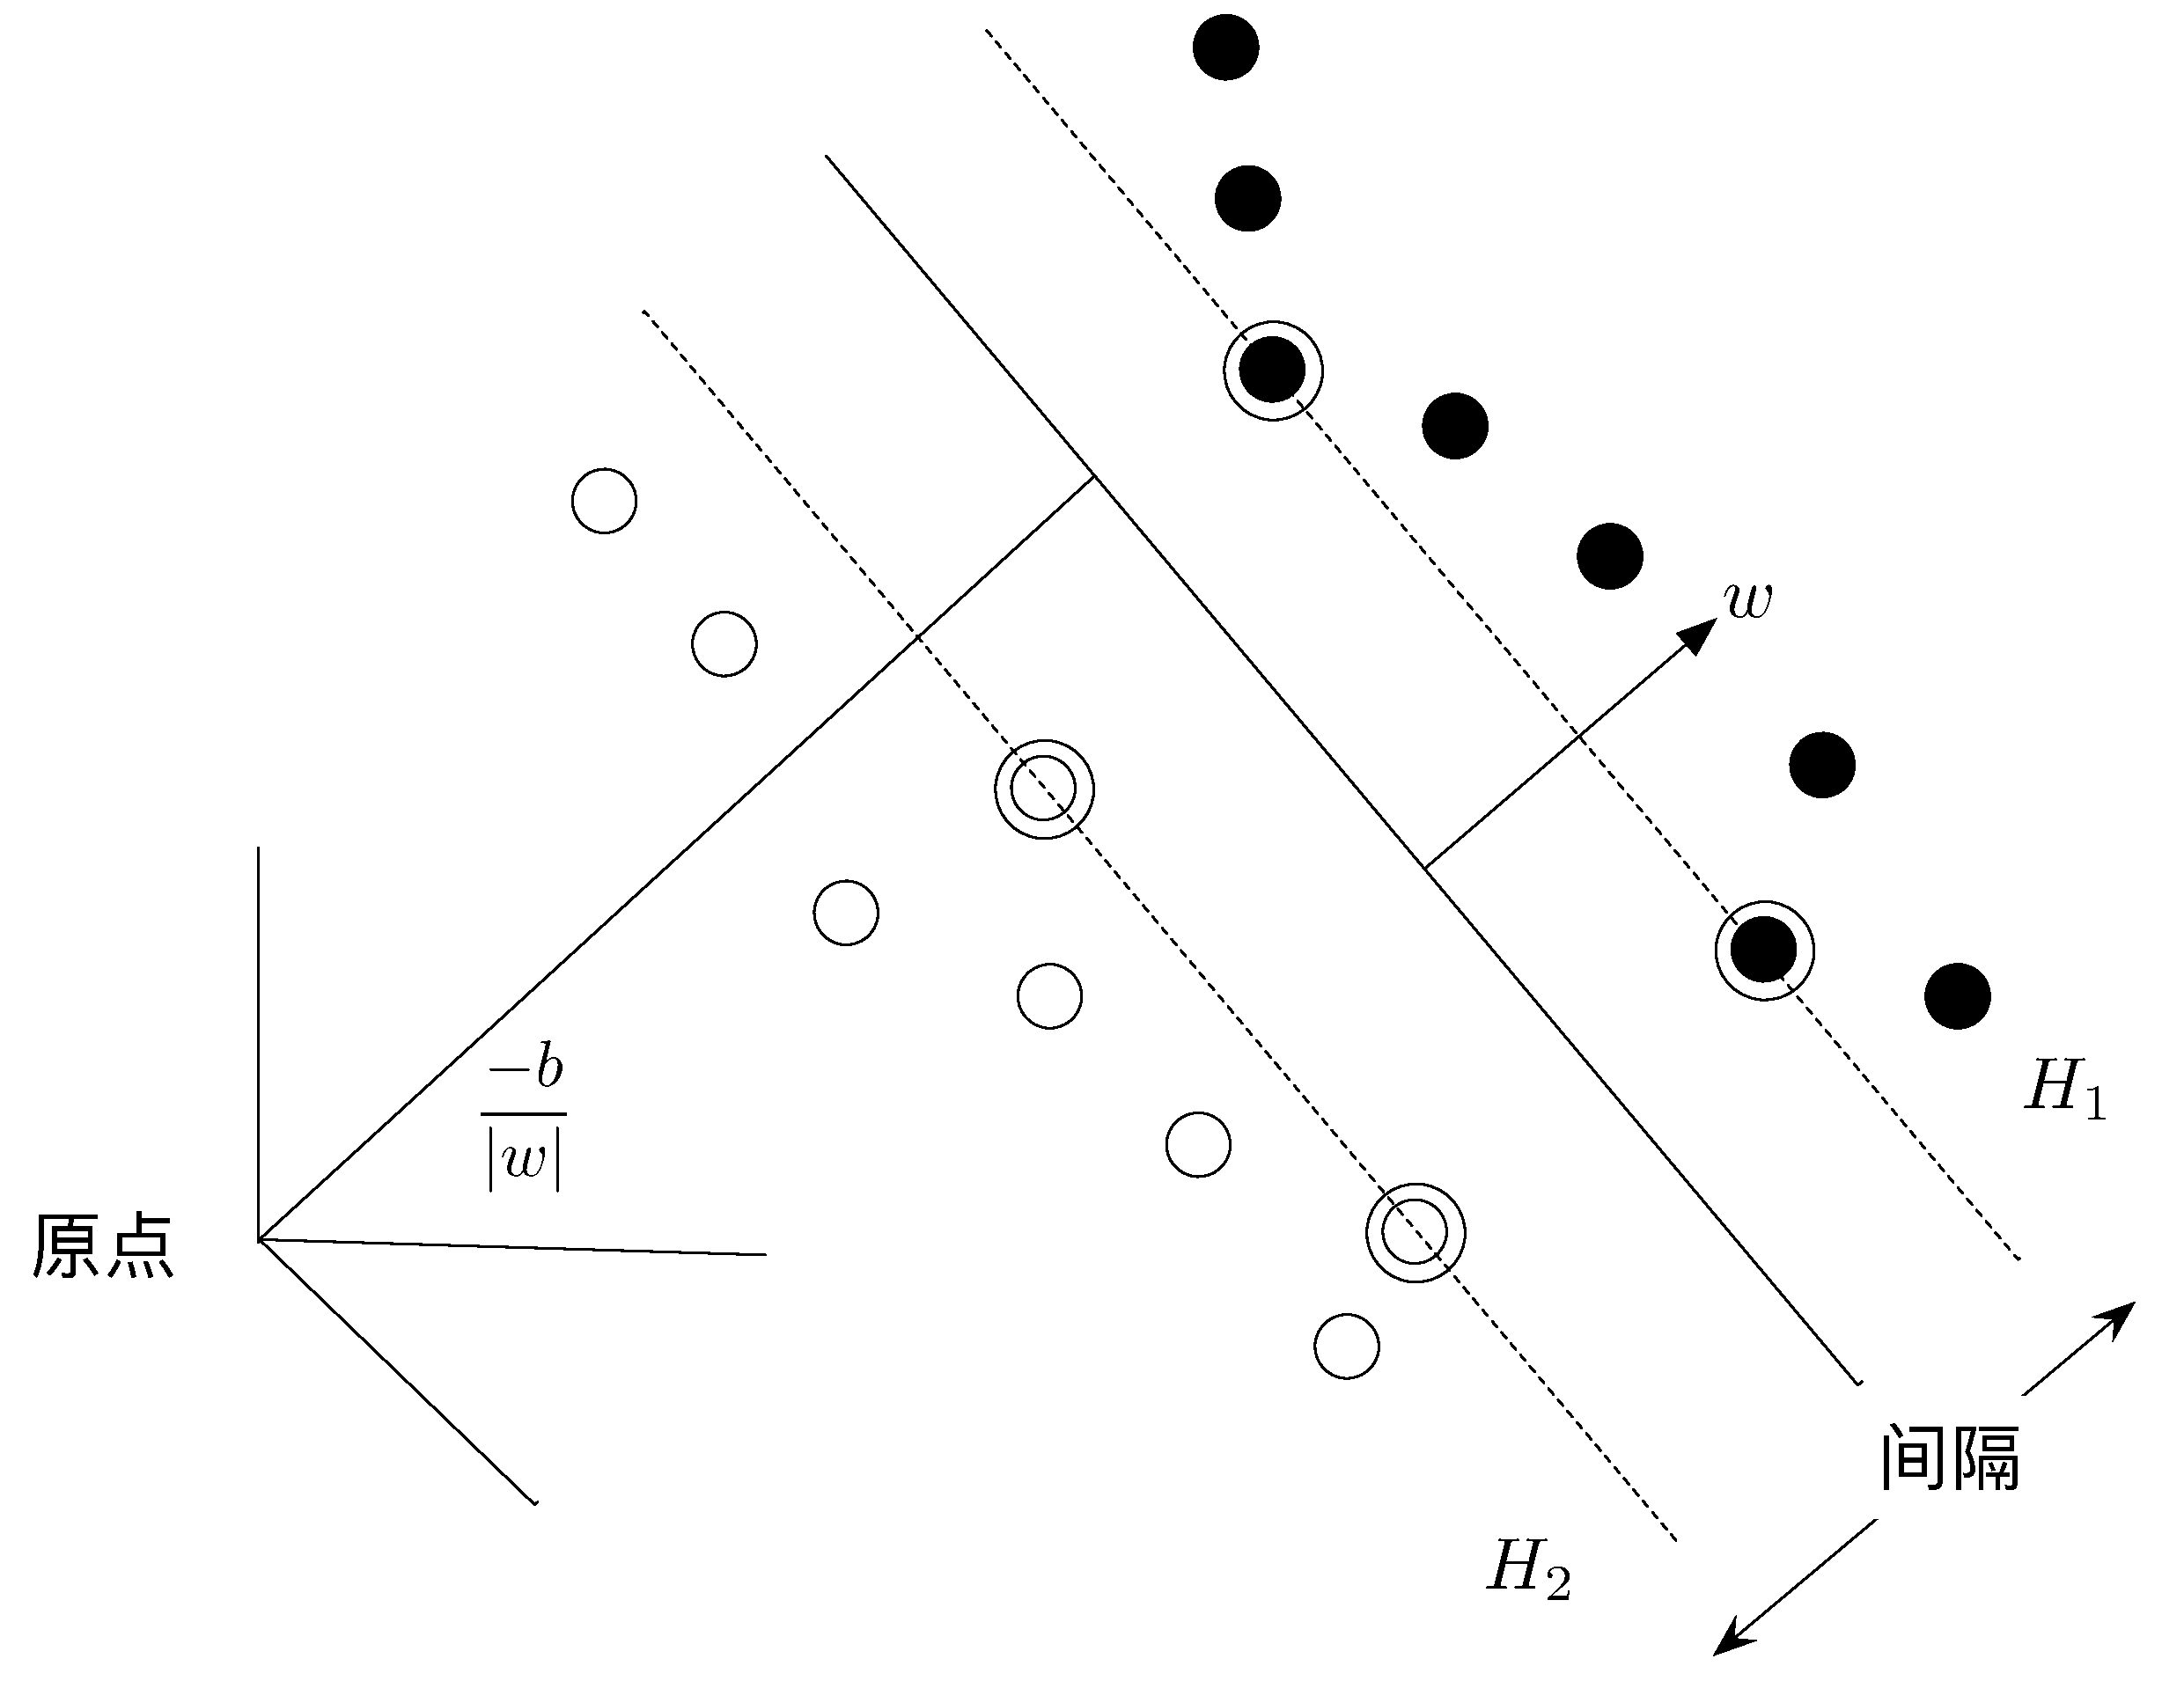
\includegraphics[width=6.67cm]{figures/emitter/svm_hard}
	\caption{标准分类平面,即具有最大间隔的超平面。被圈起来的样本组成超平面,这些样本被称作支持向量。}
	\label{fig:hyperplanes}
\end{figure}
因此求解标准分类超平面的最大间隔的问题,就转变为一个优化问题:
\begin{equation}
	\min \limits_{w\in \mathcal{H}} \tau(w)=\frac{1}{2}||w||^2\quad s.t. \quad y_i(w\cdot x_i +b) \geq 1 \quad \forall i
	\label{equ:optimization}
\end{equation}
为了更好表示约束,可以用拉格朗日优化算法对\equref{equ:optimization}重新表示:
\begin{equation}
	\min \limits_{w,b} L(w,b,\alpha)=\frac{1}{2}||w||^2-\sum_{i=1}^l\alpha_i y_i (x_i w + b) + \sum_{i=1}^l{\alpha_i},
	\label{equ:lagrange}
\end{equation}
其中$\alpha_i \geq 0$为约束条件。

在实际计算过程中,可以通过对偶定义求解优化方程\equref{equ:lagrange},通过最大化方程\equref{equ:lagrange}相对于$\alpha$来求取其相对于$w$和$b$的最小值。利用 Karush-Kuhn-Tucker 条件,\equref{equ:lagrange}变为对偶形式:
\begin{equation}
	\max \limits_{\alpha} L_D=\sum_i{\alpha_i}-\frac{1}{2}\sum_{i,j}\alpha_i\alpha_jy_iy_jx_i\cdot x_j \quad s.t. \quad \forall i
	\left\{
		\begin{aligned}
	   &\sum_i{\alpha_iy_i}=0  \\
	   &\alpha_i \geq 0
	   \end{aligned}
		\right.
\end{equation}
因此,通过求解该对偶优化问题,可以得到系数$\alpha_i$,其中满足$\alpha_i>0$的解称作支持向量,他们位于标准分类平面$H_1$或者$H_2$上。注意到,仅有$\alpha_i>0$的解影响最终的支持向量的选择。
因此,可以得到决策函数:
\begin{equation}
	f(x)=w^Tx_i+b=\sum_{i=1}^My_i\alpha_i(x_i^Tx)+b.
\end{equation}
决策函数的符号取决于预测样本$x$。

此处讨论的情形的一个假设是可以把所有样本完全分为不同的类别。但是显然在大多数情况下,这种假设是不成立的。另外,这种假设也会导致过拟合现象的出现。因此,文献 \cite{cortes1995support} 提出了软间隔的支持向量机。
其主要思想是通过引入正的松弛变量$\xi_i$放宽\equref{equ:constraint}的约束,从而得到:
\begin{equation}
	\forall i \quad
	\left\{
	 \begin{aligned}
	&w\cdot x_i + b \geq +1-\xi_i \quad y_i=+1  \\
	&w\cdot x_i + b \leq -1-\xi_i \quad y_i=+1  \\
	&\xi_i \geq 0
	\end{aligned}
	 \right.
	\label{equ:constraint_soft}
\end{equation}
这允许一些样本在边缘内部,甚至在相反类别的情况下进一步交叉(见图\ref{fig:softmargin})。 虽然这种松弛使得支持向量机能够灵活地降低异常值的影响,但是从优化问题求解的角度来看,任意大的松弛变量$\xi_i$可能会导致SVM获得平凡解或次优解。 因此,可以通过使松弛变量成为\equref{equ:optimization}的一部分,来限制松弛度:
\begin{equation}
	\min \limits_{w\in \mathcal{H},\xi\in \mathbb{R}^m} \tau(w,\xi)=\frac{1}{2}||w||^2+C\sum_{i=1}^m {\xi_i}
\end{equation}
\begin{figure}[hbt]
	\centering
	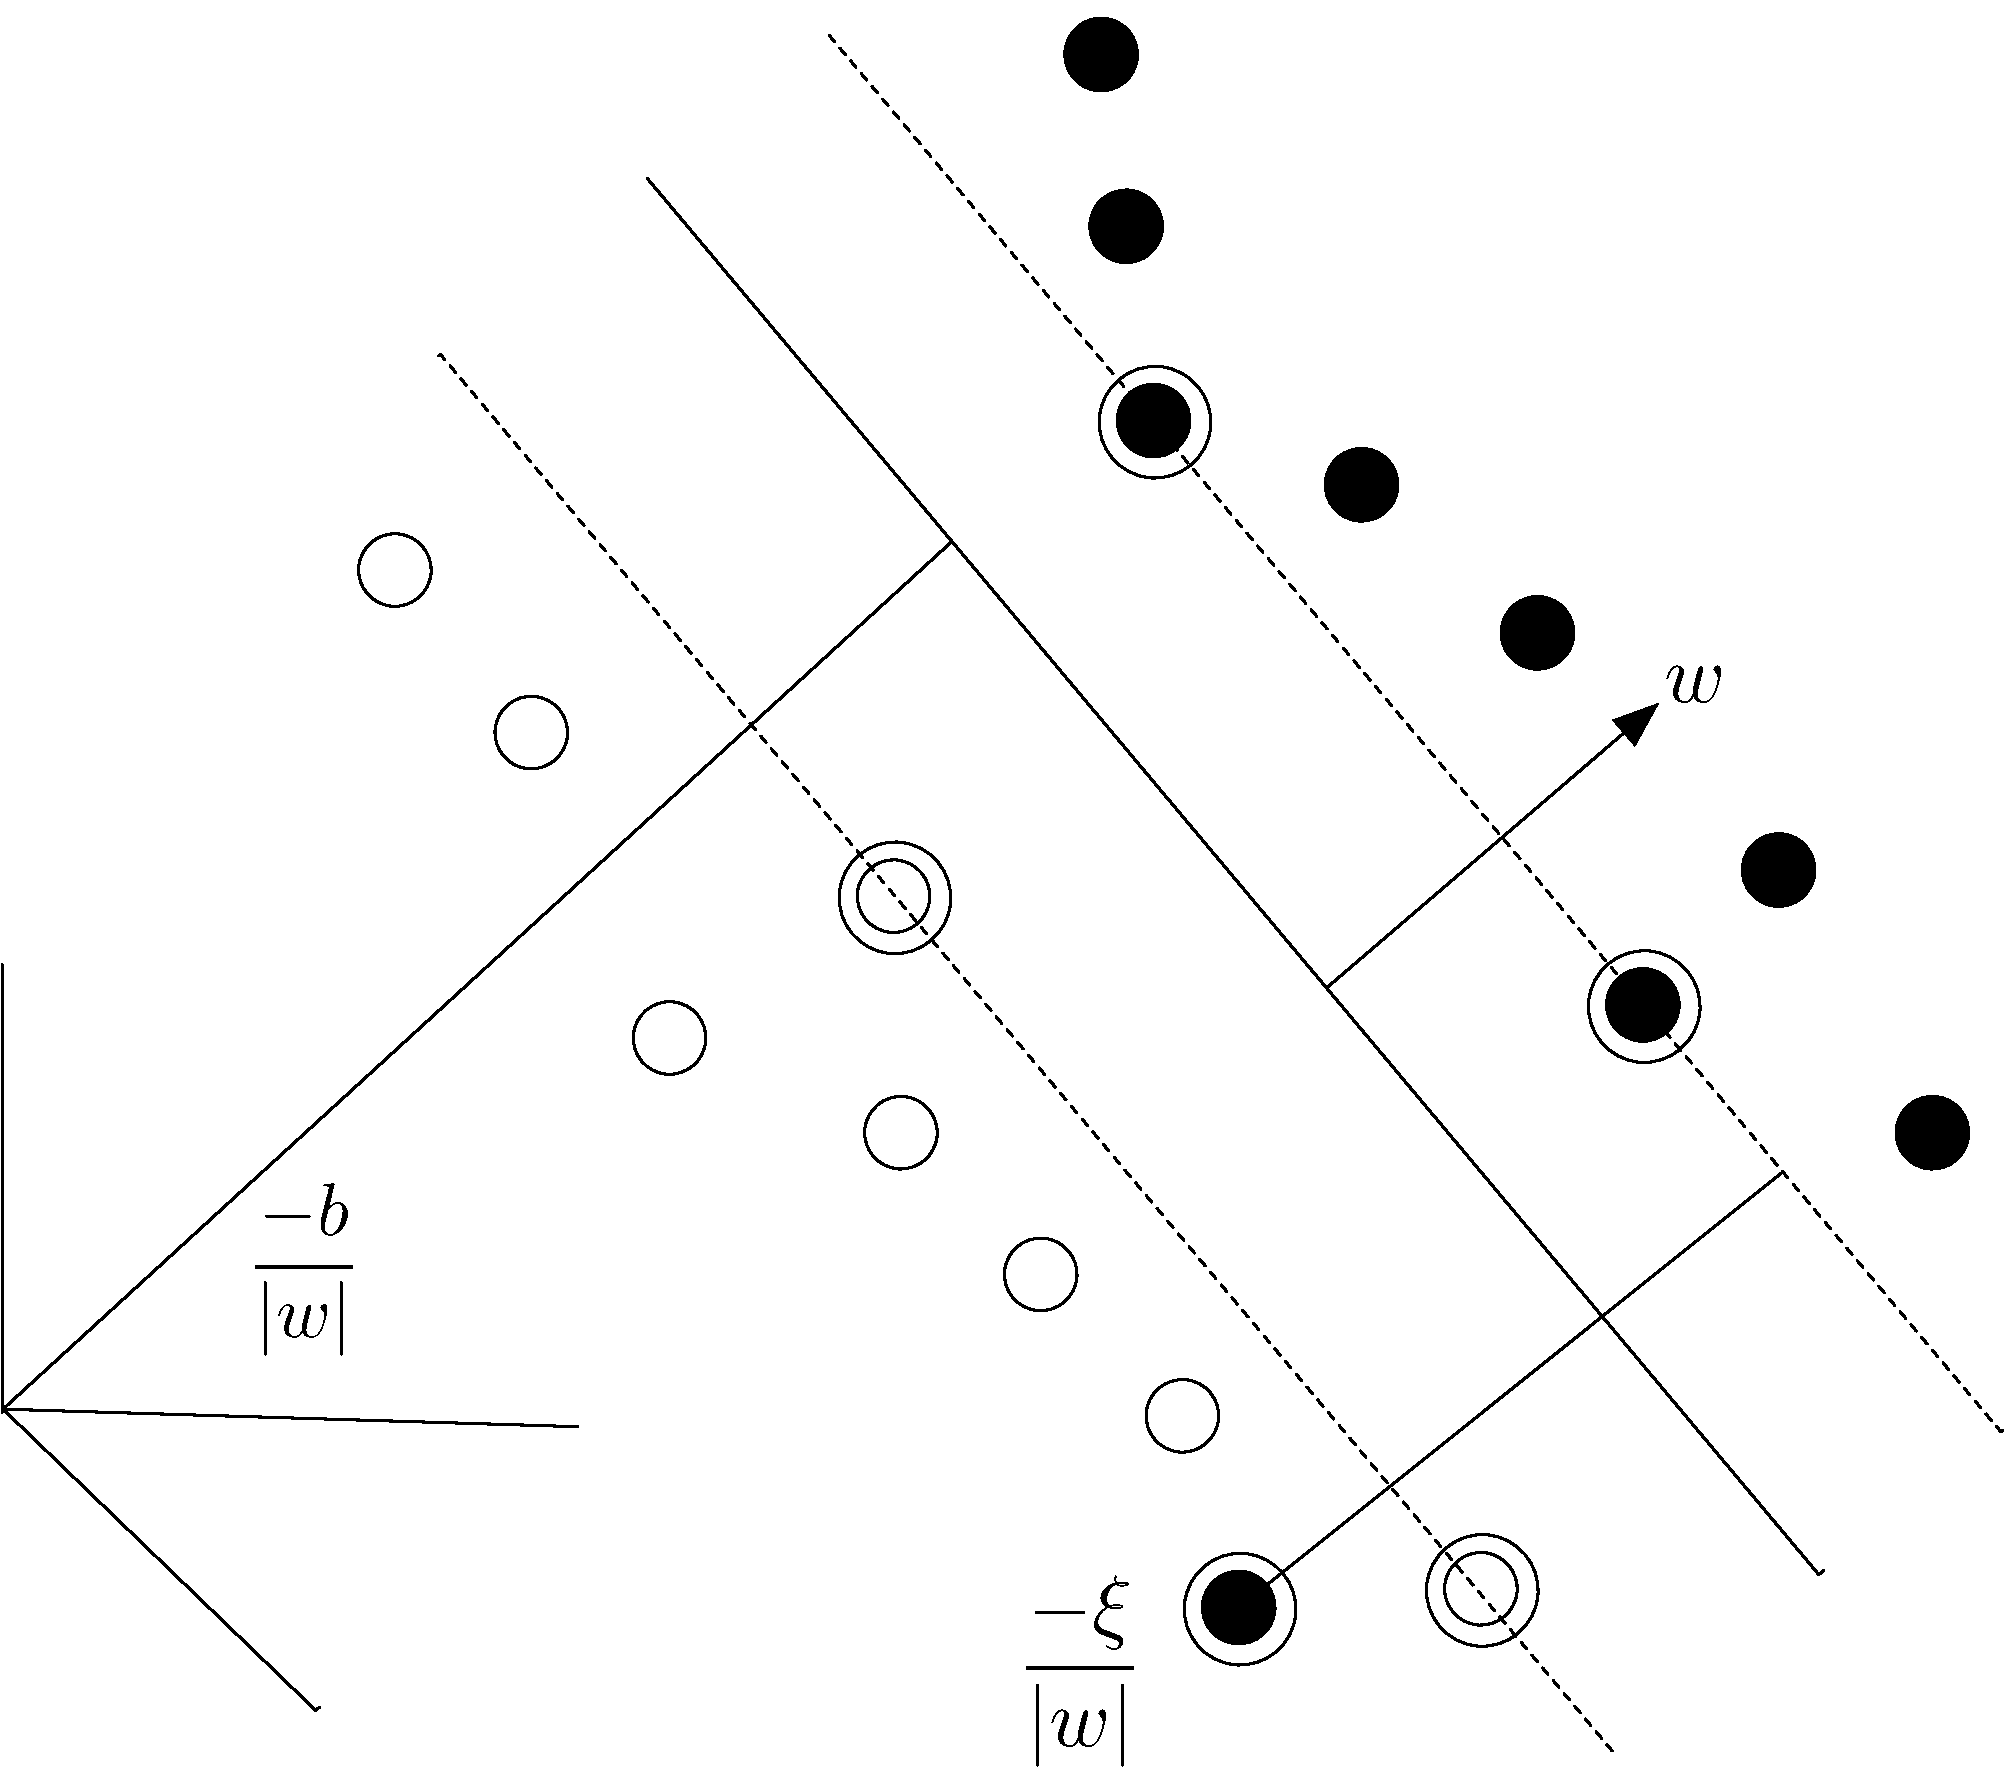
\includegraphics[width=6.67cm]{figures/emitter/svm_soft}
	\caption{软间隔支持向量机}
	\label{fig:softmargin}
\end{figure}
其约束条件为\equref{equ:constraint_soft}。超参数$C>0$是针对误分类的惩罚系数,该系数需要根据不同的分类任务和数据集进行调整,
将其变为对偶形式:
\begin{equation}
	\max \limits_{\alpha} L_D=\sum_i{\alpha_i}-\frac{1}{2}\sum_{i,j}\alpha_i\alpha_jy_iy_jx_i\cdot x_j \quad s.t. \quad \forall i
	\left\{
		\begin{aligned}
	   &\sum_i{\alpha_iy_i}=0  \\
	   &C \leq \alpha_i \geq 0
	   \end{aligned}
		\right.
	\label{equ:cdotdual}
\end{equation}
目前只是分析了线性支持向量机的问题,为了应对非线性分类问题,引入了核函数的概念。
将训练数据通过某函数$\Phi:\mathbb{R}^d\mapsto\mathcal{H}$,经过该变换后,只需要将原来计算$\mathbb{R}^d$的$x_i\cdot x_j$ 变为计算在$\mathcal{H}$域的向量积$\Phi(x_i)\cdot\Phi(x_j)$。为了降低计算量,可以引入核函数$K$来避免数据$x_i$和$x_j$从$\mathbb{R}^d$映射到$\mathcal{H}$:
\begin{equation}
	K(x_i,x_j)=\Phi(x_i)\cdot\Phi(x_j).
\end{equation}
因此,可以将\equref{equ:cdotdual}变为:
\begin{equation}
	\max \limits_{\alpha} L_D=\sum_i{\alpha_i}-\frac{1}{2}\sum_{i,j}\alpha_i\alpha_jy_iy_j K(x_i,x_j)\quad s.t. \quad \forall i
	\left\{
		\begin{aligned}
	   &\sum_i{\alpha_iy_i}=0  \\
	   &C \leq \alpha_i \geq 0
	   \end{aligned}
		\right.
\end{equation}
常用的核函数有下面几种:
\begin{itemize}
	\item 线性核函数:$K(x,y)=x^Ty+C$
	\item 多项式核函数:$K(x,y)=(x^Ty+C)^d$
	\item RBF 核函数:$K(x,y)=e^{\frac{-||x-y||^2}{2\sigma^2}}$
	\item Sigmoid 核函数:$K(x,y)=\tanh(\alpha x^Ty+C)$
\end{itemize}
\subsubsection{支持向量机设计}
本章设计的支持向量机分类器以深度卷积神经网络的输出作为输入,利用各类别的概率作为特征进行训练识别。
由于在类别的识别过程中存在一定的波动性,其会影响结果是否属于未知类别的辨别,因此本章选取来自同一个辐射源连续10拍的识别结果平均作为最终的输入。

支持向量机分类器的设计主要分为核函数的选择和参数的选择两方面。核函数将输入空间映射到高维特征空间,最终在高维特征空间中构造出最优分类超平面,从而把平面上本身不好分的非线性数据分开。常用的核函数为线性核函数和径向基核函数( Radial Basis Function, RBF)。在核函数的选择方面,当特征数量很大时一般选用线性核函数,而对本章这种特征数量比较小的问题,一般选择径向基核函数。

具有径向基核的支持向量机具有两个关键参数,惩罚参数$C$的和核参数$\sigma$,这两个参数的取值在很大程度上决定了SVM的性能的优劣。
核参数$\sigma$主要影响样本数据在高维特征空间中分布的复杂程度,即维数。特征子空间的维数越高,那么得到的最优分类超平面就会越复杂。因此只有选择合适的核参数得到合适的特征子空间,才能得到泛化能力良好的SVM分类器。大量的实验数据表明,如果与样本点之间的距离很小,$\sigma \rightarrow 0$;如果与样本点之间的距离很大时,$\sigma \rightarrow \infty$。当$\sigma$很小,径向基核函数支持向量机得到的判别函数差不多是一个常数,出现过拟合现象;当$\sigma$很大时,样本的正确分类率也会比较低。

惩罚参数是影响SVM算法性能的另一个重要因素。它的作用主要是调节特征子空间中SVM模型的置信范围与经验风险的比例,使支持向量机的泛化能力达到最好。当特征子空间不同时,最优参数值取值也会不同。惩罚参数与经验误差的惩罚和SVM的复杂度成正比,与经验风险值成反比。因此,选择合适的惩罚参数也是非常重要的。

\section{仿真实验与分析}
\label{sec:sei_experiment}
\subsection{实验环境}

本章利用了来自13架民航飞机的气象雷达辐射源的数据,飞机信息参见表\ref{tab:flight}
\begin{table}[hbt]
	\renewcommand{\arraystretch}{1.3}
	\caption{辐射源信号数据}
	\label{tab:flight}
	\centering\sWuhao
	\begin{tabularx}{\textwidth}{>{\centering\arraybackslash}X>{\centering\arraybackslash}X>{\centering\arraybackslash}X}
		\toprule
		 飞机地址码 & 飞机航班号 & 飞机型号  \\
		 \midrule
		 7BF014 & CCA1416 & Airbus A330 (twin-jet)\\
		 780DB3 & TBA9881 & Airbus A330 (twin-jet) \\
		 780E06 & CSN3438 & Airbus A330 (twin-jet\\
		 780EBB & CES293 & 	Airbus A321 (twin-jet)\\
		 780EBF & CES2342 & Airbus A320 (twin-jet)\\
		 7804F2 & ZH9164 & Airbus A320 (twin-jet)\\
		 7804F4 & CES5856 & Boeing 737\\
		 7806FC & CSN6402 & Airbus A320 (twin-jet)\\
		 7808F0 & CES5373 & Airbus A319 (twin-jet)\\
		 78057F & CCA4103 & Airbus A321 (twin-jet\\
		 780063 & CCA4377 & Airbus A319 (twin-jet)\\
		 780375 & CSC8253 & Airbus A319 (twin-jet)	\\
		 781022 & EU2731 & Airbus A319 (twin-jet)\\
		 \bottomrule
	\end{tabularx}
\end{table}

本章利用的数据是机载气象雷达辐射源信号,原始的雷达信号是如图 \ref{fig:IQ} 所示的I/Q信号,
为了更好的捕捉到雷达辐射源回波的特征信息,本章对数据进行了一个变换,利用快速傅里叶变换求取其模糊函数,并取偏移为0附近的一个切片作为输入的特征向量,经过变换后的样本的特征如图\ref{fig:diff_data}所示。
\begin{figure}[hbt]
	\centering
	\begin{minipage}{7cm}
		\centering
		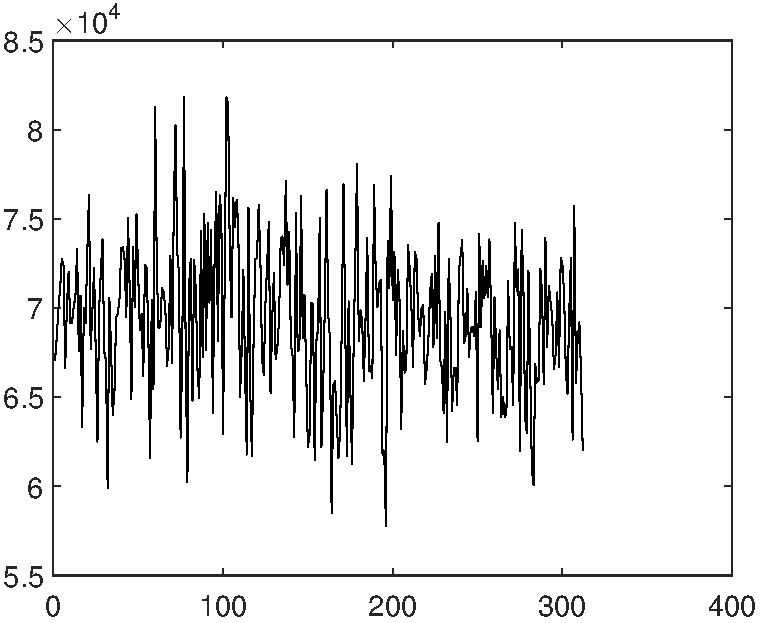
\includegraphics[width=6.67cm]{figures/emitter/IQA}
		\caption{原始I/Q信号}
		\label{fig:IQ}
	\end{minipage}
	\hspace{10pt}
	\begin{minipage}{7cm}
		\centering
		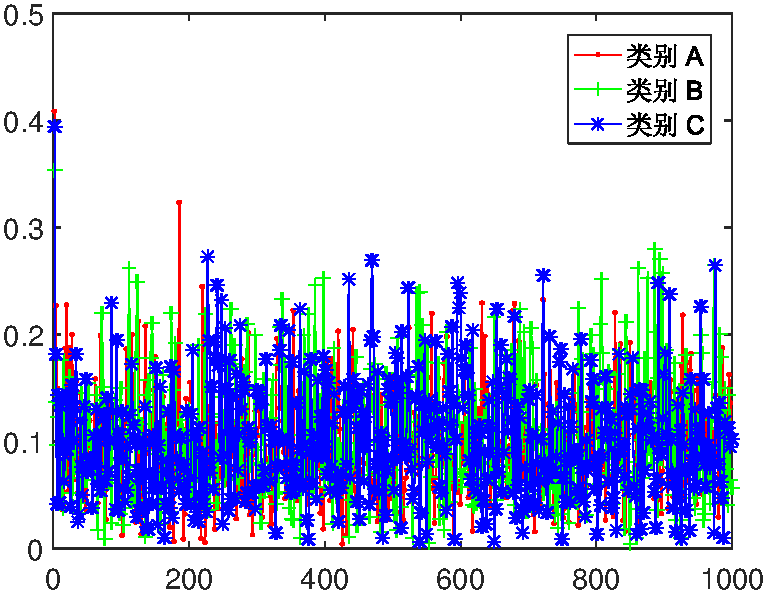
\includegraphics[width=6.67cm]{figures/emitter/diff_data}
		\caption{不同类别样本特征图}
		\label{fig:diff_data}
	\end{minipage}
\end{figure}
由于该变换后,数据之间的差距比较大,为了通过线性变换将原始数据映射到$[0 , 1]$之间
本章对数据利用离差标准化(Min-Max Normalization)方法进行归一化,
转换函数如下:
\begin{equation}
x^{*}=\frac{x-x_{min}}{x_{max}-x_{min}},
\end{equation}
其中$x_{max}$为样本数据的最大值,$x_{min}$为样本数据的最小值。

在数据的选择方面,本章从全部数据中选择出2至8个类别分别进行实验,每一个类别的原始信号为100次雷达扫描周期的信号。
由于深度学习需要大量的数据进行训练学习,而本身数据量偏少,故本章在已有数据的基础上在一定信噪比的前提下,生成部分仿真数据,最终每架飞机均有10000组信号。本章选择全部数据的$70\%$作为训练样本,$20\%$用于交叉验证,$10\%$作为测试,同时在测试样本中添加与其等量的来自未训练类别也即未知类别的样本共同作为测试样本用来衡量其未知分类的识别率。
本章采用网格搜索法对SVM参数进行调优,最终选择参数惩罚参数为$C=32$,核参数$\sigma=0.0312$。

\subsection{实验结果分析}

\subsubsection{深度卷积神经网络识别结果}

首先验证深度卷积算法的识别正确率,利用8个类别的数据进行训练和测试,迭代次数为100次,其分类结果如表\ref{tab:cnn_29}所示。从表格中容易看出,每一个单独类别的分类精度都很高。
\begin{table}[hbt]
	\renewcommand{\arraystretch}{1.3}
	\caption{深度卷积神经网络分类结果}
	\label{tab:cnn_29}
	\centering\sWuhao
	\begin{tabular}{ccccccccc}
		\toprule
		 & 类别 A & 类别 B & 类别 C & 类别 D & 类别 E & 类别 F & 类别 G & 类别 H \\
		 \midrule
		 类别 A & 100\% & 0 & 0 & 0 & 0 & 0 & 0 & 0 \\
		 类别 B & 7.42\% & 92.58\% & 0 & 0 & 0.13 & 0 & 0 & 0 \\
		 类别 C & 0 & 0 & 97.83\% & 0 & 0 & 2.17\% & 0 & 0 \\
		 类别 D & 0 & 0 & 3\% & 97\% & 0 & 0 & 0 & 0 \\
		 类别 E & 0 & 0 & 0 & 0 & 100\% & 0 & 0 & 0 \\
		 类别 F & 0 & 0 & 0.08\% & 0 & 0 & 99.92\% & 0 & 0 \\
		 类别 G & 0 & 0 & 1.08\% & 0 & 0 & 0 & 98.92\% & 0 \\
		 类别 H & 1.63\% & 0 & 0 & 0 & 0 & 0.63 & 0 & 98.37\% \\
		\bottomrule
	\end{tabular}
\end{table}

同对迭代次数与识别准确率和损失函数进行了验证,其结果如图 \ref{fig:openset_epoch}、图\ref{fig:diff_loss}和表\ref{tab:cnn_epoch_29}所示,无论是训练样本还是测试样本,其精度与损失函数均很快收敛到比较好的水平,不过相应的学习时间也正比增长,故在实际工程中需要对精度和时间进行衡量选取一个最合适的迭代次数。
\begin{table}[hbt]
	\renewcommand{\arraystretch}{1.3}
	\caption{深度卷积神经网络分类结果}
	\label{tab:cnn_epoch_29}
	\centering\sWuhao
		\begin{tabularx}{\textwidth}{>{\centering\arraybackslash}X>{\centering\arraybackslash}X>{\centering\arraybackslash}X>{\centering\arraybackslash}X}
		\toprule
		迭代次数 & 训练样本学习正确率 & 测试样本学习正确率  &  学习时间(s) \\
		 \midrule
			1 & 0.4670 & 0.5782 & $1.0931\times 10^3$ \\
			2 & 0.7658 & 0.7758 & $2.3572\times 10^3$ \\
			10 & 0.9414 & 0.8102 & $1.1444\times 10^4$ \\
			20 & 0.9709 & 0.9065 & $2.1370\times 10^4$ \\
			40 & 0.9819 & 0.9883 & $4.3181 \times 10^4$ \\
			50 & 0.9839 & 0.9830 & $5.3437 \times 10^4$ \\
			60 & 0.9866 & 0.9746 & $6.4143 \times 10^4$ \\
			70 & 0.9903 & 0.9904 & $7.4849 \times 10^4$ \\
			80 & 0.9904 & 0.9798 & $8.5597 \times 10^4$ \\
			90 & 0.9908 & 0.9872 & $9.6328\times 10^4$ \\
			100 & 0.9902 & 0.9811 & $1.0711 \times 10^5$ \\
		\bottomrule
	\end{tabularx}
\end{table}

\begin{figure}[hbt]
	\centering
	\begin{minipage}{7cm}
		\centering
		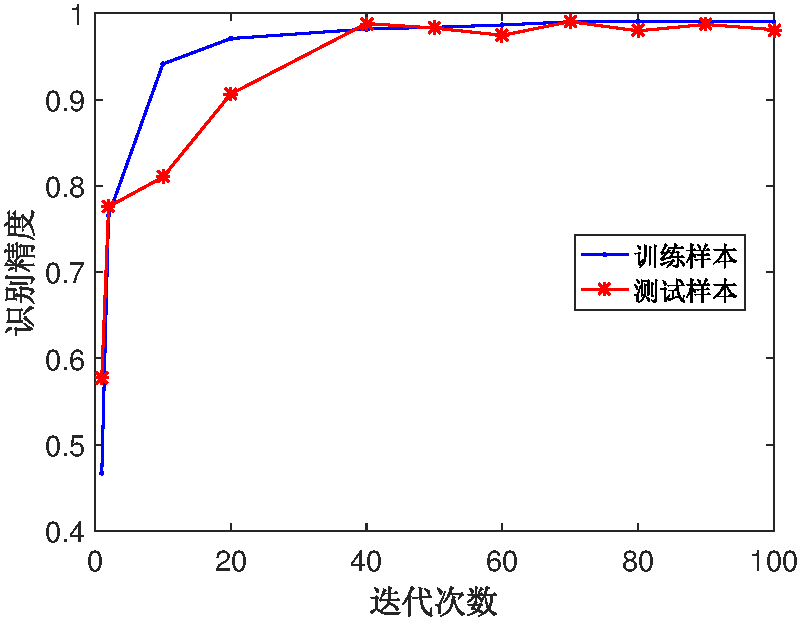
\includegraphics[width=6.67cm]{figures/emitter/diff_epoch}
		\caption{迭代次数与识别准确率曲线图}
		\label{fig:openset_epoch}
	\end{minipage}
	\hspace{10pt}
	\begin{minipage}{7cm}
		\centering
		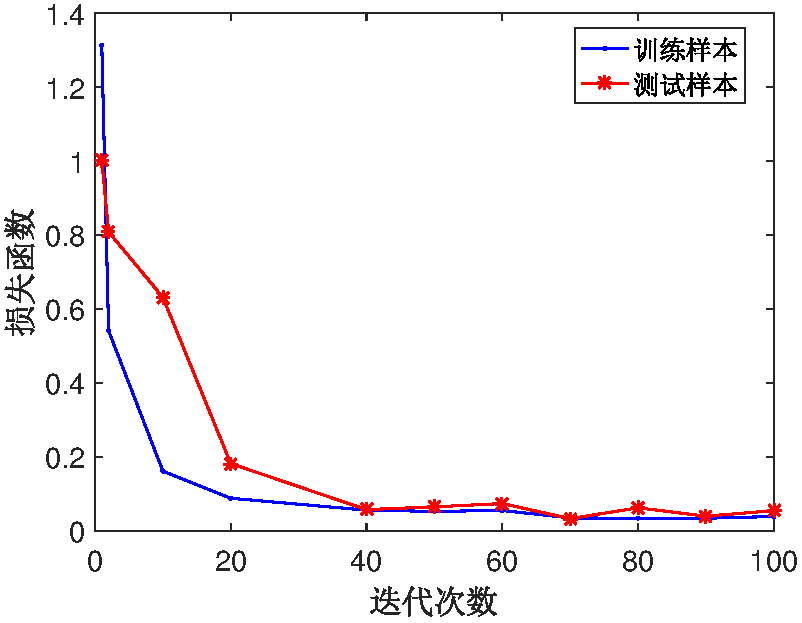
\includegraphics[width=6.67cm]{figures/emitter/diff_loss}
		\caption{迭代次数与损失函数曲线图}
		\label{fig:diff_loss}
	\end{minipage}
\end{figure}
\subsubsection{Open Set 分类器识别结果}

在上述样本的情形下,可以通过选取不同的类别数目,进行实验得到表\ref{tab:nb_classes}的识别结果。
从表中可以看出,随着样本类别数的增加,未知分类的识别准确率也随之有了大幅度的增加,同时每个类别的识别准确率仍然维持在比较高的水平。

\begin{table}[hbt]
	\renewcommand{\arraystretch}{1.3}
	\caption{不同已知类别个数数据识别结果}
	\label{tab:nb_classes}
	\centering\sWuhao
	\begin{tabularx}{\textwidth}{>{\centering\arraybackslash}X>{\centering\arraybackslash}X>{\centering\arraybackslash}X}
		\toprule
		 已知类别数目 & 已知类别识别正确率 & 未知类别分辨正确率 \\
		\midrule
		2 & 99.55\% & 84.32\% \\
		3 & 99.59\% & 93.10\% \\
		4 & 99.00\% & 97.81\% \\
		5 & 99.75\% & 98.42\% \\
		6 & 98.63\% & 98.85\% \\
		7 & 99.28\% & 99.22\% \\
		8 & 97.86\% & 99.14\% \\
		\bottomrule
	\end{tabularx}
\end{table}

\section{小结}
\label{sec:sei_summary}
本章针对复杂电磁环境下辐射源的识别面临的电磁信号干扰大、雷达信号参数相近等问题与挑战,利用深度学习的思想与方法,深入研究辐射源脉内细微特征,设计合适的深度卷积神经网络结构和支持向量机Meta-Recognition,实现了对辐射源中未知分类的辨别。基于民航机载气象雷达数据对本章提出的方法进行初步验证,表明该方法具有较强的抗噪声、抗干扰能力以及较好的鲁棒性。
% 传统方法进行辐射源个体识别前均需进行降噪、多径抑制和分选等复杂的信号预处理工作,这些操作会在一定程度上削弱雷达的个体特征。通过对现有辐射源信号进行分析,深度学习方法利用其脉内细微特征作为训练样本,使得识别准确率有了较大的进步。
